\documentclass[tikz]{standalone}
\usepackage{tikz}
\usetikzlibrary{positioning, graphs}
\usetikzlibrary{graphs.standard}
\usetikzlibrary{arrows.meta}
\begin{document}
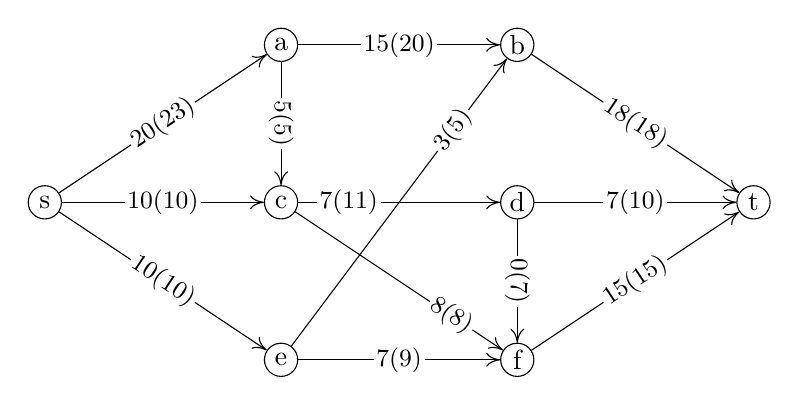
\begin{tikzpicture}
\begin{scope}
		[vertex/.style={draw,circle,inner sep = 0em, minimum size = 1.2em},
		 edgelabel/.style = {fill = white, inner sep = 0.1em, font=\small, sloped}]
		\node[vertex] (s) at (0,0) {s};
		\node[vertex] (a) at (3,2) {a};
		\node[vertex] (b) at (6,2) {b};
		\node[vertex] (c) at (3,0) {c};
		\node[vertex] (d) at (6,0) {d};
		\node[vertex] (e) at (3,-2) {e};
		\node[vertex] (f) at (6,-2) {f};
		\node[vertex] (t) at (9,0) {t};
		
		\draw[-{>[length=5, width=5]}] (s) to node[edgelabel] {$20(23)$} (a);
		\draw[-{>[length=5, width=5]}] (s) to node[edgelabel] {$10(10)$} (c);
		\draw[-{>[length=5, width=5]}] (s) to node[edgelabel] {$10(10)$} (e);
		\draw[-{>[length=5, width=5]}] (a) to node[edgelabel] {$15(20)$} (b);
		\draw[-{>[length=5, width=5]}] (a) to node[edgelabel] {$5(5)$} (c);
		\draw[-{>[length=5, width=5]}] (c) to node[edgelabel, near start] {$7(11)$} (d);
		\draw[-{>[length=5, width=5]}] (c) to node[edgelabel, near end] {$8(8)$} (f);
		\draw[-{>[length=5, width=5]}] (e) to node[edgelabel, near end] {$3(5)$} (b);
		\draw[-{>[length=5, width=5]}] (e) to node[edgelabel] {$7(9)$} (f);
		\draw[-{>[length=5, width=5]}] (b) to node[edgelabel] {$18(18)$} (t);
		\draw[-{>[length=5, width=5]}] (d) to node[edgelabel] {$0(7)$} (f);
		\draw[-{>[length=5, width=5]}] (d) to node[edgelabel] {$7(10)$} (t);
		\draw[-{>[length=5, width=5]}] (f) to node[edgelabel] {$15(15)$} (t);		
\end{scope}
\end{tikzpicture}
\end{document}